\documentclass[t]{beamer}
\usetheme{Copenhagen}
\setbeamertemplate{headline}{} % remove toc from headers
\beamertemplatenavigationsymbolsempty

\usepackage{amsmath, array, tikz, tcolorbox, bm, tkz-euclide, pgfplots, graphicx}
\pgfplotsset{compat = 1.16}
\usetkzobj{all}
\everymath{\displaystyle}

\title{Parabolas}
\author{}
\date{}

\AtBeginSection[]
{
  \begin{frame}
    \frametitle{Objectives}
    \tableofcontents[currentsection]
  \end{frame}
}

\begin{document}

\begin{frame} 
\maketitle
\end{frame}

\begin{frame}[c]
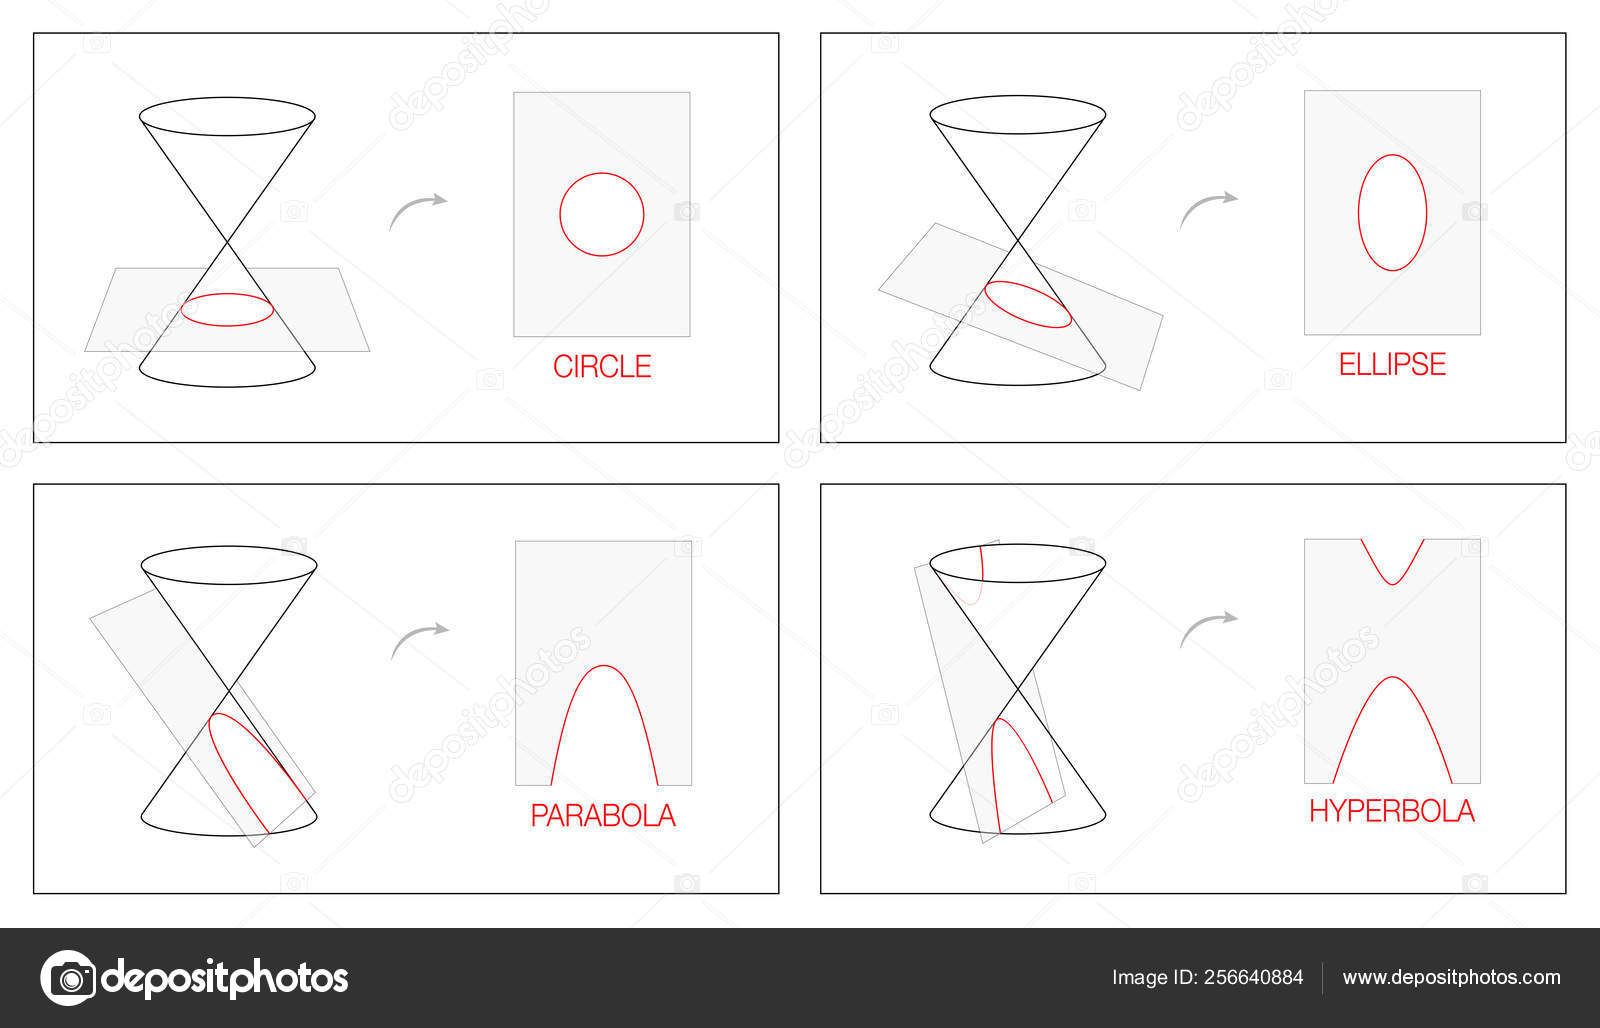
\includegraphics[scale=0.80]{Images/conics.jpg}
\end{frame}

\section{Identify vertex, focus, and directrix from an equation.} 

\begin{frame}{Parabolas}
If we look at the graph of the quadratic function $f(x) = ax^2 + bx + c$, we obtain what is known as a \emph{parabola}.	\newline\\	\pause

\begin{tcolorbox}[colback=red!10!white, colframe=red!60!black,, title=\textbf{Parabolas}]
The set of all points in the plane that are the same distance from the focus and the directrix line.
\end{tcolorbox}
\end{frame}

\begin{frame}{Parabolas}
\begin{center}
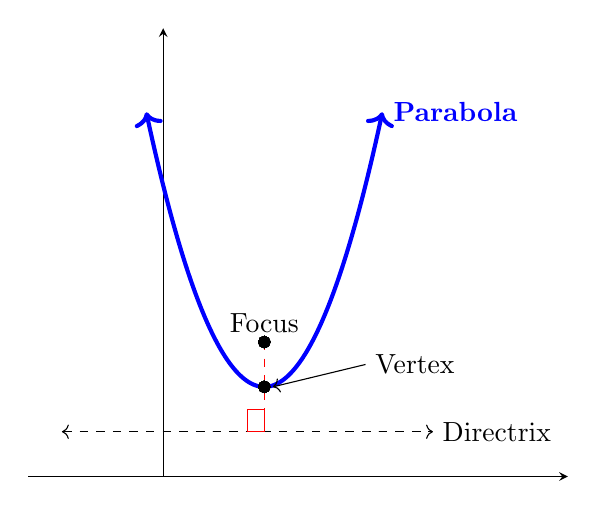
\begin{tikzpicture}
    \begin{axis}[
    axis lines = middle,
    xmin = -4,
    xmax = 12,
    ymin = 0,
    ymax = 10,
    xtick = \empty,
    ytick = \empty]
    \addplot [color=blue, <->, samples=200, domain=-0.5:6.5, line width = 1.5] {2 + 0.5*(x-3)^2} node[right]{\color{blue}{\textbf{Parabola}}};
    \addplot [mark = *] (3, 3) node[above]{Focus};
    \addplot [dashed, <->, samples=200, domain = -3:8] {1} node[right]{Directrix};
    \addplot [mark = *] (3, 2);
    \draw [<-] (3.25,2) -- (6,2.5) node[right]{Vertex};
    \draw [color=red] (3,1) rectangle (2.5,1.5);
    \draw [color=red, dashed] (3,3) -- (3,2) -- (3,1);
    \end{axis}
\end{tikzpicture}
\end{center}
\end{frame}

\begin{frame}{General Form of a Parabola}
The general form of a parabola is the familiar quadratic equation $f(x) = ax^2 + bx + c$.	\newline\\	\pause
The {\color{blue}\textbf{vertex forms}} of a parabola are given below.

\begin{center}
    \setlength{\extrarowheight}{7pt}
    \begin{tabular}{c|c|c}
    &   \textbf{Opens Up or Down}   &   \textbf{Opens Left or Right}    \\  \hline
    &   $y = a(x-h)^2 + k$  &   $x = a(y-k)^2 + h$  \\[5pt]  \hline
    Vertex  &   $(h,k)$ &   $(h,k)$ \\[5pt]  \hline
    Focus   &   $(h,k+p)$ where $a = \frac{1}{4p}$   &   $(h+p,k)$ where $a = \frac{1}{4p}$  \\[5pt] \hline
    Directrix   &   $y = k-p$   &   $x = h-p$   \\
    \end{tabular}
\end{center}
\end{frame}

\begin{frame}{General Form of a Parabola}
\emph{Note}: $p$ is the distance from the focus to the vertex, or the distance from the vertex to the directrix; either interpretation is correct.	\newline\\

\begin{center}
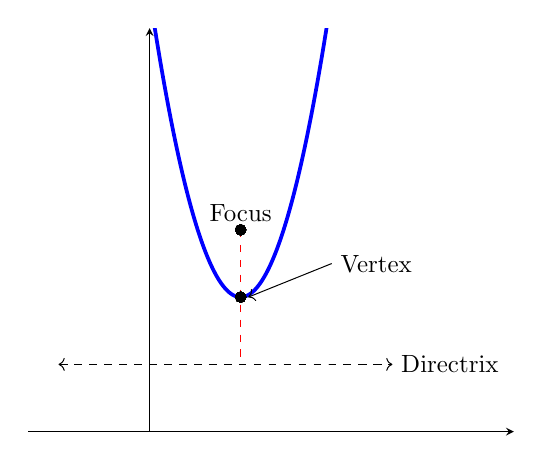
\begin{tikzpicture}[scale=0.9]
    \begin{axis}[
    axis lines = middle,
    xmin = -4,
    xmax = 12,
    ymin = 0,
    ymax = 6,
    xtick = \empty,
    ytick = \empty]
    \addplot [color=blue, <->, samples=200, domain=-0.5:6.5, line width = 1.5] {2 + 0.5*(x-3)^2} node[right]{\color{blue}{\textbf{Parabola}}};
    \addplot [mark = *] (3, 3) node[above]{Focus};
    \addplot [dashed, <->, samples=200, domain = -3:8] {1} node[right]{Directrix};
    \addplot [mark = *] (3, 2);
    \draw [<-] (3.25,2) -- (6,2.5) node[right]{Vertex};
    \draw [color=red, dashed] (3,3) -- (3,2) -- (3,1);
    \end{axis}
\end{tikzpicture}
\end{center}
\end{frame}

\begin{frame}{Example 1}
Identify the vertex, focus, and directrix for each of the following.    \newline\\  
(a) \quad $ y = 2(x+1)^2 $	\newline\\
\onslide<2->{Vertex: $(-1,0)$}	\newline\\
\onslide<3->{Focus:
\begin{align*}
\frac{1}{4p} &= 2	\\[8pt]
\onslide<3->{1 &= 8p} \\[6pt]
\onslide<4->{p &= \frac{1}{8}}
\end{align*}
}
\end{frame}

\begin{frame}{Example 1 \quad Vertex: $(-1,0)$, $p = \tfrac{1}{8}$}
Focus: $\left(-1, 0 + \frac{1}{8}\right)$		
\onslide<2->{\qquad $= \left(-1,\frac{1}{8}\right)$} \\[10pt]
\onslide<3->{Directrix: $y=-\frac{1}{8}$}
\end{frame}

\begin{frame}{Example 1}
(b)	\quad	$y = -0.25(x-3)^2 + 4$	\newline\\
\onslide<2->{Vertex: $(3,4)$} \newline\\
\onslide<3->{Focus:
\begin{align*}
\frac{1}{4p} &= \frac{1}{4}	\\[10pt]
\onslide<4->{4p &= 4} \\[8pt]
\onslide<5->{p &= 1}
\end{align*}
}
\end{frame}

\begin{frame}{Example 1 \quad Vertex: $(3,4)$, $p=1$}
Focus: $(3,4-1)$	
\onslide<2->{\qquad $=(3,3)$}	\\[8pt]
\onslide<3->{Directrix: $y = 5$}
\end{frame}

\begin{frame}{Example 1}
(c)	\quad $x = 2(y+7)^2 - 9$	\newline\\
\onslide<2->{Vertex: $(-9,-7)$}	\newline\\
\onslide<3->{Focus:
\begin{align*}
\frac{1}{4p} &= 2 \\[10pt]
\onslide<4->{1 &= 8p} \\[8pt]
\onslide<5->{p &= \frac{1}{8}}
\end{align*}
}
\end{frame}

\begin{frame}{Example 1 \quad Vertex: $(-9,-7)$, $p = \tfrac{1}{8}$}
Focus: $\left(-9+\frac{1}{8}, -7\right)$
\onslide<2->{\qquad $=\left(-\frac{71}{8}, -7\right)$}		\\[11pt]
\onslide<3->{Directrix: $x = -\frac{73}{8}$}
\end{frame}

\begin{frame}{Example 1}
(d)	\quad	$x = -3y^2$	\newline\\
\onslide<2->{Vertex: $(0,0)$}	\newline\\
\onslide<3->{Focus:
\begin{align*}
\onslide<4->{\frac{1}{4p} &= 3} \\[10pt]
\onslide<5->{1 &= 12p} \\[10pt]
\onslide<6->{p &= \frac{1}{12}}
\end{align*}
}
\end{frame}

\begin{frame}{Example 1 \quad Vertex: $(0,0)$, $p = \tfrac{1}{12}$}
Focus: $\left(0-\frac{1}{12}, 0\right)$	
\onslide<2->{\qquad $=\left(-\frac{1}{12}, 0\right)$} \\[10pt]
\onslide<3->{Directrix: $x = \frac{1}{12}$}
\end{frame}


\section{Find the equation given vertex, focus, and/or directrix.}


\begin{frame}{How To}
This is just working backwards from the previous section. Having any two of the three pieces of information is sufficient enough to create the equation for that parabola.
\end{frame}

\begin{frame}{Example 2}
Find the equation of each parabola given the following information.	\newline\\
(a)	\quad	Focus $(0, -3)$, directrix $y = 3$	\newline\\
\onslide<2->{Vertex: $(0,0)$}	\newline\\
\onslide<3->{$p = 3$} 	
\begin{align*}
\onslide<4->{a &= \frac{1}{4p}} \\[10pt]
\onslide<5->{a &= \frac{1}{4(3)}} \\[10pt]
\onslide<6->{a &= \frac{1}{12}}
\end{align*}
\end{frame}

\begin{frame}{Example 2a \quad Vertex: $(0,0)$, $a = \tfrac{1}{12}$}
Since parabola opens down, $a = -\frac{1}{12}$	
\begin{align*}
\onslide<2->{y &= -\frac{1}{12}\left(x-0\right)^2 + 0} \\[11pt]
\onslide<3->{y &= -\frac{1}{12}x^2}
\end{align*}
\end{frame}

\begin{frame}{Example 2}
(b)	\quad	Focus $(-1,1)$, directrix $x = -3$	\newline\\
\onslide<2->{Vertex: $(-2,1)$}	\newline\\
\onslide<3->{$p = 1$}
\begin{align*}
\onslide<4->{a &= \frac{1}{4p}} \\[10pt]
\onslide<5->{a &= \frac{1}{4(1)}} \\[10pt]
\onslide<6->{a &= \frac{1}{4}}
\end{align*}
\end{frame}

\begin{frame}{Example 2b \quad Vertex: $(-2,1)$, $a = \tfrac{1}{4}$}
Since parabola opens right, $a = \frac{1}{4}$	\\[10pt]
\onslide<2->{\[x=\frac{1}{4}\left(y-1\right)^2-2\]}
\end{frame}

\begin{frame}{Example 2}
(c)	\quad Vertex $(2,1)$, focus $(2,3)$	\newline\\
\onslide<2->{$p = 2$} \\[10pt]
\begin{align*}
\onslide<3->{a &= \frac{1}{4p}} \\[10pt]
\onslide<4->{a &= \frac{1}{4(2)}} \\[10pt]
\onslide<5->{a &= \frac{1}{8}}
\end{align*}
\end{frame}

\begin{frame}{Example 2c \quad Vertex: $(2,1)$, $a=\tfrac{1}{8}$}
Since parabola opens up, $a = \frac{1}{8}$	\\[12pt]
\onslide<2->{\[y = \frac{1}{8}\left(x-2\right)^2+1\]}
\end{frame}

\begin{frame}{Example 2}
(d)	\quad	Vertex $(3,-1)$, focus $(2,-1)$	\newline\\
\onslide<2->{$p=1$}		\\[10pt]
\begin{align*}
\onslide<3->{a &= \frac{1}{4p}} \\[10pt]
\onslide<4->{a &= \frac{1}{4(1)}} \\[10pt]
\onslide<5->{a &= \frac{1}{4}}
\end{align*}
\end{frame}

\begin{frame}{Example 2d \quad Vertex: $(3,-1)$, $a = \tfrac{1}{4}$}
Since parabola opens to the right, $a = -\frac{1}{4}$	\\[11pt]
\onslide<2->{\[x = -\frac{1}{4}\left(y+1\right)^2+3\]}
\end{frame}


\section{Convert parabolas from general to vertex form.}

\begin{frame}{Quadratic Expressions}
This is revisiting writing quadratic expressions written in general form to standard form. 	\newline\\	\pause

This is also known as \alert{completing the square}
\end{frame}

\begin{frame}{Example 3}
Write each in vertex form.	\newline\\
(a)	\quad $y = -\frac{1}{4}x^2 + 5x - 24$	\newline\\
\onslide<2->{Vertex: $(10, 1)$} \newline\\
\onslide<3->{$a = -\frac{1}{4}$} \newline\\
\onslide<4->{\[y = -\frac{1}{4}\left(x-10\right)^2 + 1\]}
\end{frame}

\begin{frame}{Example 3}
(b)	\quad $y = -x^2-4x-14$	\newline\\
\onslide<2->{Vertex: $(-2, -10)$} \newline\\
\onslide<3->{$a = -1$} \newline\\
\onslide<4->{\[y = -\left(x+2\right)^2 - 10\]}
\end{frame}

\begin{frame}{Example 3}
(c)	\quad $x=\frac{1}{2}y^2+7y+\frac{41}{2}$	\newline\\
\onslide<2->{Vertex: $(-4, -7)$} \newline\\
\onslide<3->{$a = \frac{1}{2}$} \newline\\
\onslide<4->{\[x = \frac{1}{2}\left(y+7\right)^2 - 4\]}
\end{frame}

\begin{frame}{Example 3}
(d)	\quad $x=-y^2-2y+9$	\newline\\
\onslide<2->{Vertex: $(10, -1)$} \newline\\
\onslide<3->{$a = -1$} \newline\\
\onslide<4->{\[x = -(y+1)^2 + 10\]}
\end{frame}

\end{document}